\section{Methods}

\begin{figure}[h]
    \centering
    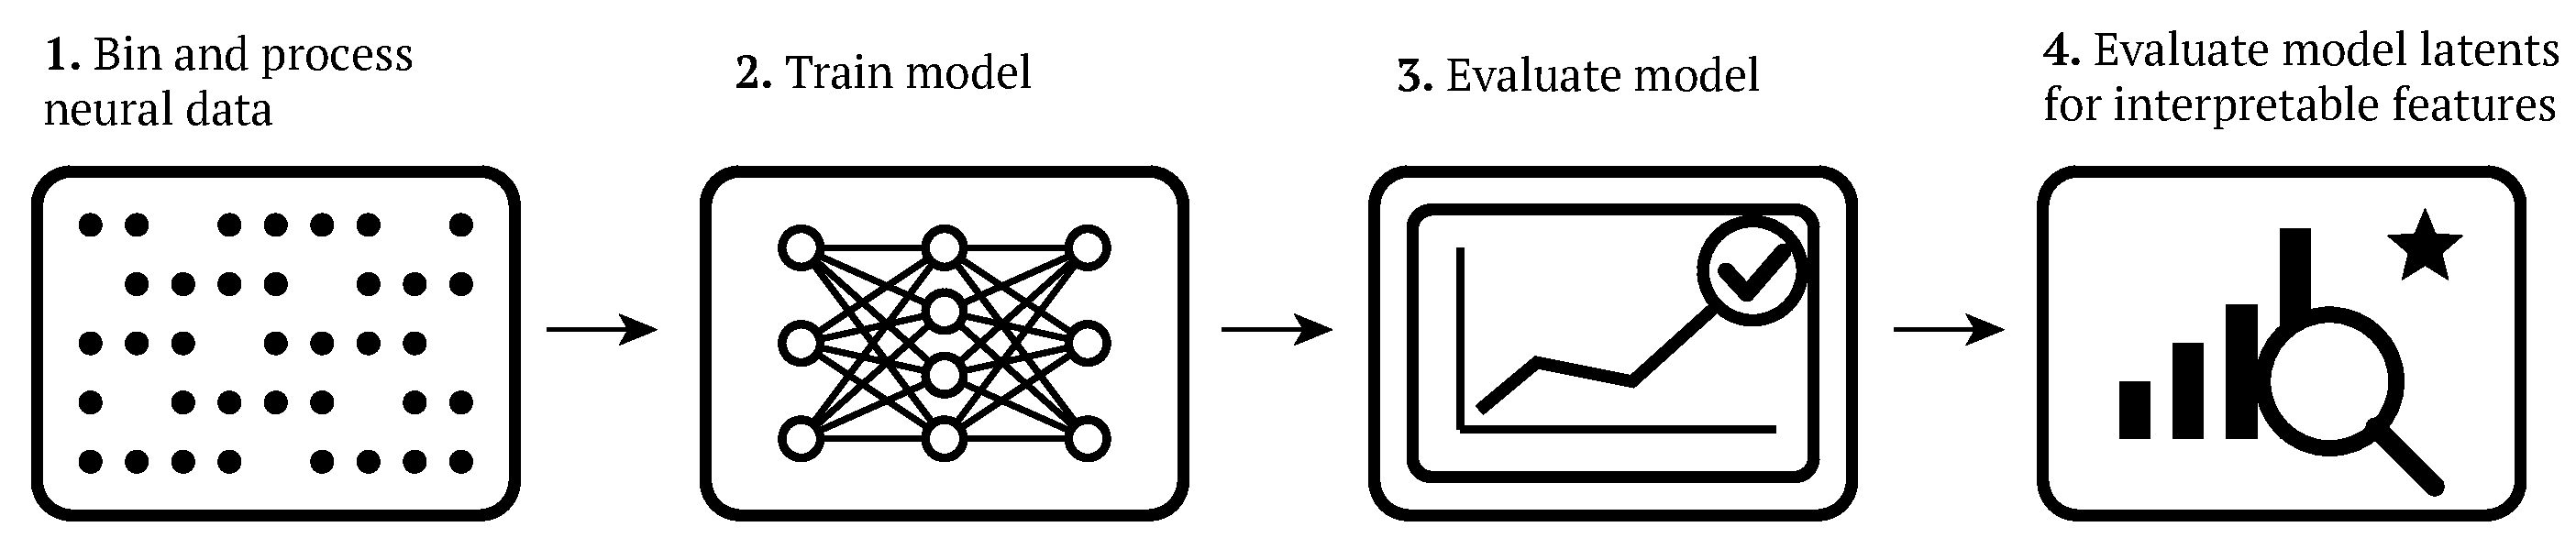
\includegraphics[width=\linewidth]{figures/mini_pipeline.pdf}
    \caption{
        \textbf{The MINI pipeline.} \\
        \small The MINI pipeline is comprised of 4 steps: 1) Spatiotemporal binning and processing of neural data; 2) Model training; 3) Model evaluation (and optional re-training); 4) Latent evaluation for feature interpretability. Steps 1-3 including model re-training, can be either semi- or fully-automated.
    }
    \label{fig:mini_pipeline}
\end{figure}

MINI takes in high-dimensional neural data and outputs interpretable latents. The semi-automated pipeline consists of four steps (\autoref{fig:mini_pipeline}), the first three of which can be fully automated.

In step 1, data processing is performed to prepare the neural data for model training. MINI contains code to take the output from common spikesorters (e.g. Kilosort ~\cite{pachitariu_2016_kilosort}), bin it into a 2D matrix of time X space (e.g. timebins, units (putative neurons)), and normalize the data (e.g. max normalize or z-score normalize across space (e.g. units) or time (e.g. timebins)). Users can also manually bin and process their neural data before proceeding to step 2.

- A similar approach could be applied to output from common calcium imaging processing tools (e.g. Suite2p ~\cite{pachitariu_2017_suite2p}).

In step 2, a SDNN model is trained on the processed neural data. This model reconstructs the data from sparsely active dictionary elements, with the goal of having these elements correspond to natural features encoded by the neural activity, thereby producing readily interpretable latents (\autoref{fig:sdnn_arch} \textbf{a}, \textbf{b}). For example, when a model is trained on neural activity from visual cortex, an element may correspond to a particular property of a stimulus in the visual field, and similarly, when a model is trained on neural activity from the motor cortex, an element may correspond to a particular quality of movement. 

The model can be configured as an autoencoder, transcoder, or crosscoder ~\cite{lindsey_2024_crosscoders}, depending on whether the to-be-reconstructed target neural activity is the same as (e.g. we are trying to reconstruct V2 activity with the same 21 activity as input), dependent on (e.g. we are trying to reconstruct V2 activity with V1 activity as input), or otherwise related to (e.g. we are trying to reconstruct V2 activity from subject1 based on V2 activity from subject2 from a given timepoint in a given task to see if they have shared representations) the input neural activity, respectively.

MINI employs a novel variant of the Matryoshka SDNN architecture ~\cite{bussmann_2025_msae} to segment the latent space into multiple hierarchical levels, with each level attempting a full reconstruction of the target neural activity (\autoref{fig:sdnn_arch} \textbf{c}). This allows for multi-feature representation at a single point in time. e.g. we can have neural representations for a round object, a ball, and most specifically, a basketball, when we see one. A key feature of SDNN models is the fact that latents are sparsely active. Here we enforce sparsity with a batch topk approach ~\cite{bussmann_2024_batchtopk}, meaning we only keep the top $k \times batch_size$ most active latents for each input batch. This allows the number of latents active on any given example to vary, while keeping an expected mean, and ensuring we don't have to tune a separate sparsity penalty parameter.

- The novely comes from a transformer decoder layer...

- Show latex formulas for encoder, decoder, total loss.

- Model training can be set to run with a sweep, after which multiple models are evaluated in the subsequent pipeline step. The common model hyperparameters to sweep over are n\_levels, dsae\_levels, topk, and latent space sequence length. Depending on the optimizer used, it's recommended to additionally sweep over hyperparameters such as learning rate (we use Adam by default bc...)

(For additional details on model architecture and training, see \nameref{subsection:additional_pipeline_details}.)

\begin{figure}[h]
    \begin{minipage}{0.63\linewidth}
    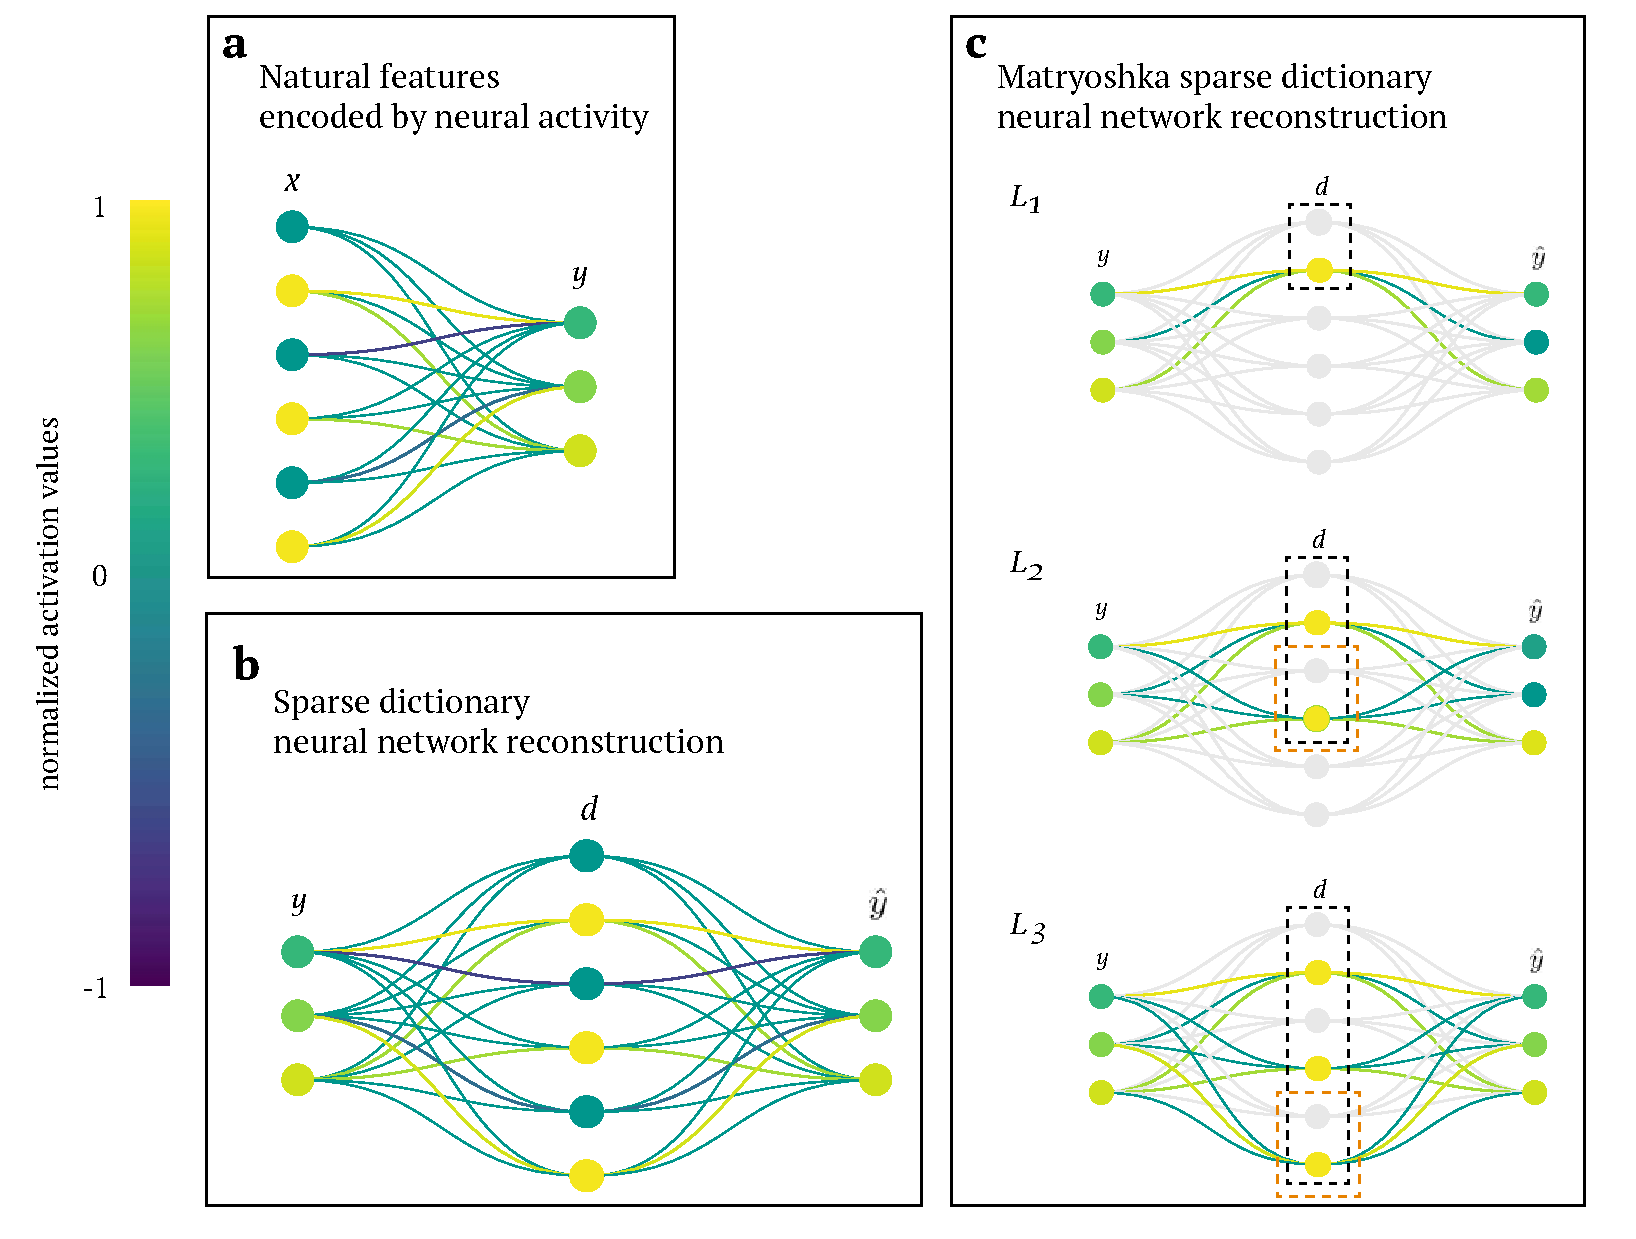
\includegraphics[width=\linewidth]{figures/sdnn_arch.pdf}
    \end{minipage}%
    \begin{minipage}{0.37\linewidth}
    \caption{
        \textbf{Model motivation} \\
        \small
        (\textbf{a}) Natural, "real-world" features $x$ are encoded by neural activity $y$. In this example, three active features are simultaneously represented by the joint activity of three neurons. (\textbf{b}) A SDNN reconstructs neural activity $z$ based on $y$ via sparse dictionary elements $d$. When training is successful, $d$ corresponds to $x$: sparse dictionary elements (i.e. model neurons) represent natural features. If $z$ tries to recreate $y$ exactly ($\hat{y}$), the model is an autoencoder; in other scenarios (e.g. $z$ is separate but dependent on or related to $y$) it is a transcoder or crosscoder. (\textbf{c}) A Matryoshka spare dictionary neural network segments the latent space into multiple levels, each of which attempts to do a full reconstruction of the target neural activity. The black boxes indicate the latents involved in a single level, while the light red boxes indicate the additional latents used at lower-levels. Additionally, for each level here we illustrate imposing a topk of 1 for each level, where only 1 latent (the most active) is chosen for reconstruction at each level. Latents in the highest-level will often correspond to high-level features (e.g. a round object), while latents exclusive to the lowest-level will often correspond to low-level features (e.g. a basketball).
    }
    \label{fig:sdnn_arch}
    \end{minipage}
\end{figure}

In step 3, the trained model is evaluated using a variety of metrics to assess its performance. (SAEBench) If the model does not meet the desired criteria, it can be re-trained with different hyperparameters. 

\begin{figure}[h]
    \centering
    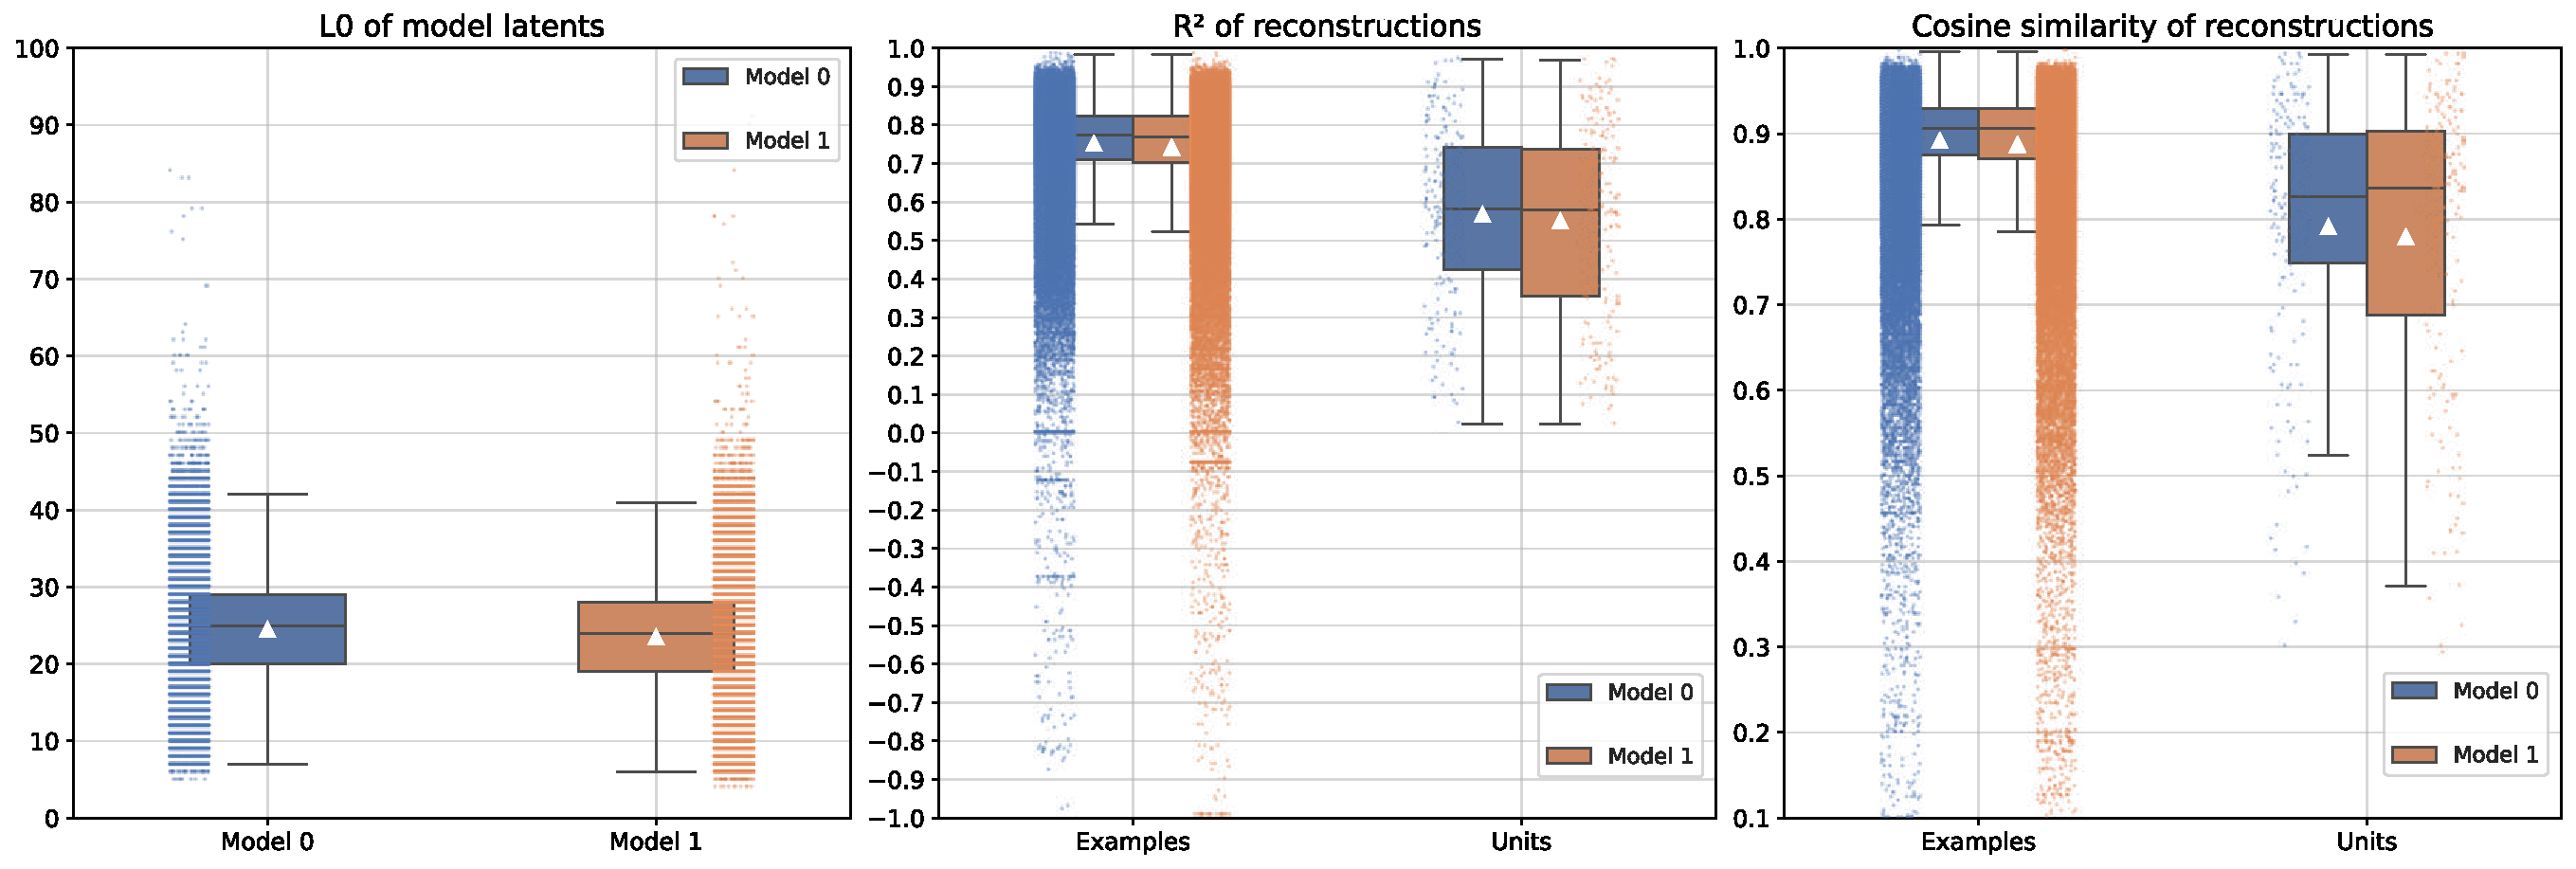
\includegraphics[width=\linewidth]{figures/model_eval.pdf}
    \caption{
        \textbf{Model evaluation metrics.} \\
        \small By default, trained models are evaluated via the following metrics: latent L0 (left), and R\textsuperscript{2} (middle) and cosine similarity (right) of reconstruction-to-actual neural activity for each temporal ("Examples") and spatial ("Units") bin. ... Additional features, such as the R\textsuperscript{2}of overall neural data reconstruction for each individual latent, can be specifed and included.
    }
    \label{fig:model_eval}
\end{figure}

Finally, in step 4, the latents produced by the model are evaluated for interpretability as features. This includes visualizing their activation patterns over time and experimental conditions, as well as assessing their decoding performance. We detail typical approaches to feature evaluation in \nameref{section:results}.

- For a user, the full, semi-automated pipeline is as follows:
\begin{enumerate}
    \item Data processing
    \begin{itemize}
        \item Spatiotemporally bin and normalize
        \begin{itemize}
            \item MINI has a convenience function to do this directly from output of common spikesorters (kilosort), where we bin unit spikes given a specified timebin and optionally normalize (z-score or max) dataset across time and/or unit
            \begin{itemize}
                \item (and similar approach could be applied to output from common calcium imaging processing (e.g. Suite2p))
            \end{itemize}
        \end{itemize}
    \end{itemize}
    
    \item Model training
    \begin{itemize}
        \item Hyperparameter optimization
        \begin{itemize}
            \item Model parameters
            \item Optimizer parameters
        \end{itemize}
        \item By default no validation set, but can be added if we want to e.g. apply to other recordings of same animal, though this is not generally recommended (just train a freshie)
    \end{itemize}
    
    \item Model evaluation
    \begin{itemize}
        \item (We implement all metrics from SAEBench which are not language-model specific, plus a couple of our own)
        \item L0 of latents
        \item R\textsuperscript{2} (var explained) and cos sim of reconstruction-to-actual neural activity for each spatial bin, and each temporal bin
        \item Latent density histogram (as in SAEBench)
        \item Variance explained of overall reconstruction from each latent (variance shouldn't be in just a few features) ?
        \item Spectral frequency analysis to ensure temporal frequency content is preserved?
    \end{itemize}
    
    \item Feature evaluation
    \begin{itemize}
        \item When a latent is subjectively determined to be sufficiently interpretable, we call this a feature.
        \item Interactive plots showing feature activation patterns across time and experimental conditions.
        \item We evaluate its decoding performance?
        \item Export functionality.
    \end{itemize}
\end{enumerate}


